\documentclass[10pt]{article}
\usepackage{style/cookbook}
\usepackage{amsmath}
\usepackage{algorithm}
\usepackage{algorithmic}
\usepackage[T1]{fontenc}
\usepackage{xcolor}
\usepackage{datetime2}

\title{Cookbook}
\date{}
\author{주성호}

\begin{document}
\thispagestyle{plain}
\cfoot{\thepage}
\maketitle
{\sffamily\tableofcontents}
\newpage

\section*{Open problem}
\begin{ginzabox}[Tail of hypergeometric distribution]
If we estimate the maximum from the sampled subset of the population, what is the tail probability of the cardinality of a set whose value is greater than the estimated maximum?

\vspace*{4mm}

{\scriptsize \DTMdisplaydate{2025}{6}{17}{}}
\end{ginzabox}
\section{Random Variable Control}
\subsection{Maximum of i.i.d gaussian} 
Let $\xi_1, \dots, \xi_k$ be $k$ independent samples from $\mathcal{N}(0,1)$. Then 
\begin{equation}
    \E \left[ \max \set{\xi_1^2, \dots, \xi_k^2} \right] \leq 2 \log (2k)
\end{equation}
\subsection{Union bound for partial sums}  
\header{Etemadi's inequality} 
Let $X_1, \dots, X_n$ be independent random variables. For $i \in [n]$, let $Y_i = \sum_{j=1}^i X_j$ denote the partial sum up to $i$. Then for all $\alpha \geq 0$, 
\begin{equation}
    \Pr [\max_{i=1}^n |Y_i| > 3 \cdot \alpha] \leq 3 \cdot \max_{i=1}^n \Pr [|Y_i| > \alpha]. 
\end{equation}
\emph{Proof Sketch.} $\pr[|Y_i| > \alpha]$ term을 얻기 위해서 $|Y_i-Y_n|$과 $|Y_i|$ 사이의 independence를 사용함. 그리고 partial sum의 maximum과 각 partial sum을 연결하기 위해서 $i$번 째 partial sum이 처음으로 $3 \alpha$ 보다 큰 event로 분해함. \href{https://x.com/shortstein/status/1584879368597213185/photo/1}{(Detail)} 

\subsection{Random Singed Summation Bound} 
\header{Khintchine ineqaulity}  Let $\set{\varepsilon_n}_{n=1}^N$ be i.i.d. Rademacher random variables. Let $0 < p < \infty$ and let $x_1, \dots, x_N \in \complex$. Then 
\begin{equation}
    A_p \left( \sum_{n=1}^N |x_n|^2 \right)^{1/2} \leq \left( \E \abs{ \sum_{n=1}^N \varepsilon_n x_n}^p \right)^{1/p} \leq B_p \left( \sum_{n=1}^N |x_n|^2 \right)^{1/2}
\end{equation}
\subsection{Summation Bound} 
\header{Marcinkiewicz-Zygmund ineqaulity}  If $X_i$, $i=1, \dots, n$ are independent random variables with $\E[X_i] = 0$ and $\E[\abs{X_i}^p], 1< p < +\infty$, then 
\begin{equation}
    A_p \E \left[ \left( \sum_{i=1}^n \abs{X_i}^2 \right)^{p/2}\right] \leq \E \left[ \abs{\sum_{i=1}^n X_i }^p \right] \leq B_p \E \left[ \left( \sum_{i=1}^n \abs{X_i}^2 \right)^{p/2} \right]
\end{equation}
where $A_p$ and $B_p$ are positive constants, which depend only on $p$.  
for some constants $A_p, B_p$ depending only on $p$. 
\\~\\
\header{Latala's inequality} If $p \geq 2$ and $X, X_1, \dots, X_n$ are i.i.d. mean $0$ random variables, then we have
\begin{equation}
    \norm{\sum_{i=1}^n X_i}_{L^p} \sim \sup \set{\frac{p}{s} \left(\frac{n}{p}\right)^{1/s} \norm{X}_{L^s} \given \max \set{2, \frac{p}{n}} \leq s \leq p}
\end{equation}
\subsection{Concentraion ineqaulity}
\subsubsection{Bernstein's ineqaulity}
Let $X_1, \dots X_n$ be independent random variables. Assume $\E[X_i] = 0, \E[X_i^2] = \sigma_i^2$, and $\Pr [ |X_i| \leq 1] = 1$ for each $i \in [n]$. Let $\sigma^2 :=\sum_{i=1}^n \sigma_i^2$. Then for all $t \geq 0$, 
\begin{equation}
    \Pr \left[ \sum_{i=1}^n X_i \geq t \right] \leq \exp \left( \frac{-3t^2}{6 \sigma^2 + 2t} \right) 
\end{equation}
\emph{Proof Sketch.} First bound the MGF of each $X_i$ using taylor expansion. Then use Markov inequality for $\Pr \left[ \sum_{i=1}^n X_i \geq t \right]$ with $\exp(\lambda \cdot)$ and minimize the upper bound with $\lambda$. Then use the following lemma to finish the proof. \\~\\
\header{Lemma} Let $v > -1$. Then $(1+v) \log (1+v) \geq v + \frac{3v^2}{2v+6}$ \\ 

\subsubsection{Matrix version Bernstein's inequality} 
Let $\mB$ a fixed $q \by d$ matrix. Construct $q \by d$ matrix $\mR$ such that 
\begin{equation}
    \E [\mR] = \mB, \quad \norm{\mR}_{\text{op}} \leq L 
\end{equation}
Form the matrix sampling estimator 
\begin{equation}
    \bar{\mR}_m = \frac{1}{m} \sum_{i=1}^m \mR_i,
\end{equation}
where each $\mR_i$ is an independent copy of $\mR$. Then for every $t >0$, the estimator satisfies 
\begin{equation}
    \pr \left[ \norm{\bar{\mR}_m - \mB}_{\text{op}} \geq t \right] \leq (q+d) \cdot \exp \left( \frac{-m t^2}{m_2 (\mR) + 2Lt /3} \right),
\end{equation}
where $m_2 (R)$ is the second moment $m_2(\mR) = \max \set{ \norm{\E[\mR^* \mR]}_{\text{op}}, \norm{\E[\mR \mR^*]}_{\text{op}} }$.  \\ 

\subsubsection{Hoeffding's inequality}
Let $X_1, \dots, X_n$ be independent random variables such that $a_i \leq X_i \leq b_i$ a.s. Then for all $t >0$, 
\begin{equation}
    \pr({S_n - \E[S_n] \geq t}) \leq \exp \left( - \frac{2t^2}{\sum_{i=1}^n (b_i -a_i)^2} \right),  
\end{equation}
where $S_n = X_1 + \dots X_n$. Also, consider a set of $r$ i.i.d. random variables $X_1. \dots X_r$ such that $- \Delta \leq X_i \leq \Delta$ and $\E[X_i] = 0 $ for each $i \in [r]$. Let $\sum_{i=1}^r X_i$. Then for any $\alpha \in (0,1/2)$
\begin{equation}
    \pr [ |M| > \alpha] \leq 2 \exp( -\frac{\alpha^2}{2 r \Delta^2})
\end{equation} 
The proof uses the following: \\ 

\header{Lemma} Let $X$ be any real-valued random variable such that $a \leq X \leq b$ a.s. Then. for all $\lambda \in \real$, 
\begin{equation}
    \E [e^{\lambda (X - \E[X])}] \leq \exp \left( \frac{\lambda^2 (b-a)^2}{8} \right) 
\end{equation}
\memo{COOL FACT: conditional expectation also works for the lemma.}

\header{Variance-only form}  Consider a set of $r$ independent random variables $X_1, \dots X_r$. Let $M = \sum_{i=1}^r X_i$. Then for $\alpha \in (0,2 \var [M] / (\max_i |X_i - \E [X_i]|)) $
\begin{equation}
\pr [ \abs{M - \E [M]} > \alpha] \leq 2 \exp \left( \frac{- \alpha^2}{4 \sum_{i=1}^r \var [X_i]} \right). 
\end{equation}

\subsubsection{Paley-Zygmund inequality}  
If $Z \geq 0$ is a random variable with finite variance, and if $0 \leq \theta \leq 1$, then 
\begin{equation}
    \pr({Z > \theta \E[Z]}) \geq (1- \theta)^2 \frac{\E [Z]^2}{\E[Z^2]}
\end{equation}
\subsubsection{Max of independent Gaussians}
Let $X_1, X_2, \dots, X_n$ i.i.d. $\cN(0,1)$, then
\begin{equation}
    \E[ \max(X_1, \dots, X_n)] = \sqrt{2 \log (n)} + o (\sqrt{\log (n)})
\end{equation}
\subsubsection{DKW inequality}
DKW inequality provides a bound on the worst-case distance of empirical CDF and the true CDF: 
\begin{equation}
    \pr \left( \sup_{x \in \real} | F_n (x) - F(x)| > \varepsilon \right) \leq C e^{- 2n \varepsilon^2} \quad \mtext{for every} \varepsilon >0.
\end{equation}
For multivariate case, let $X_1, X_2, \dots, x_n$ be an i.i.d. sequence of $k$-dimensional vectors, 
\begin{equation}
    \pr\left( \sup_{t \in \real^k} | F_n (t) - F(t)  | > \varepsilon \right) \leq (n+1) k e^{-2n \varepsilon^2}
\end{equation}
for every $\varepsilon, n , k >0$. \\~\\  
Also see \href{https://x.com/ccanonne_/status/1785118388911775796/photo/1}{local DKW inequality}
\\~\\
\href{https://x.com/shortstein/status/1798864427174986096/photo/1}{Steinke version} Let $X_1, \dots, X_n$ be independent random variables with CDF $f(v) := \pr[X_i \leq v]$ for all $i \in [n]$ and $v \in \real$. Let the empirical CDF be $F_x (v): = \frac{1}{n} \sum_{i=1}^n \mathbf{1}[X_i \leq v]$ for all $v \in \real$. Then, for all $\beta >0$, 
\begin{equation}
    \pr_X \left[ \sup_{v \in \real} F_X (v) - f(v) \leq \sqrt{\frac{2 \log (1/ \beta)}{n}} + \frac{\log (1/ \beta)}{2n} \right] \geq 1- \beta.
\end{equation}
\header{Lemma} For all $t, \lambda >0$, 
\begin{equation}
    \pr \left[ \sup_{v \in \real} F_x (v) \log \left(1 + \frac{t}{f(v)} \right) > \frac{\lambda}{n} \right] \leq (1+t)^n e^{-\lambda} \leq e^{tn - \lambda}. 
\end{equation}
Note: maximum이 bound되는 event 확률 구할 때는 martingale construction해서 optional stopping theorem적용하는 것도 좋음 ㅋ Lemma에서는 bionamial exponent에 놓아서 martingale 만듬.  
\subsubsection{Quadratic form}
\header{Definition (Subgaussian random variable)} A centered random variable $X$ is said to be $v$-subgaussian if its cumulant generating function is subquadratic:
\begin{equation}
    \xi_X (t) \leq \frac{1}{2} v t^2 \quad \forall t \in \real 
\end{equation}
\header{Hanson-Wright tail bound} Let $\vx$ be a random vector with independent centered $v$-subgaussian entries and let $\mA$ be a square matrix. Then 
\begin{equation}
\prob \left( \abs{\vx^{\top} \mA \vx - \E [ \vx^{\top} \mA \vx] } \geq t \right) \leq 2 \exp \left( - \frac{c \cdot t^2}{v^2 \norm{\mA}_F^2 + v \norm{A}t}  \right),
\end{equation}
where $c>0$ is a constant independent of $v,\vx,t$ or $\mA$. 
\subsubsection{Gaussian CCDF bound}
\begin{equation}
    1 - \Phi (w) \leq \min \set{\frac{1}{2}, \frac{1}{w \sqrt{2 \pi}}} e^{-w^2 /2}, \quad w > 0 
\end{equation}
\subsubsection{McDiarmid's inequality}
A function $f : \cX \times \cX \times \dots \cX_n \to \real$ satisfies the bounded differences property if substituting the value of the $i$th coordinate $x_i$ changes the value of $f$ by at most $c_i$. More formally, if there are constants $c_1, c_2, \dots, c_n$ such that for all $i \in [n]$, and all $x_i \in \cX_1, x_2 \in \cX_2, \dots, x_n \in \cX_3$, 
\begin{equation}
    \sup_{x_i^{\prime} \in \cX_i} | f(x_1, \dots, x_{i-1}, x_i, x_{i+1}, \dots, x_n) - f(x_1, \dots, x_{i-1}, x_i^{\prime}, x_{i+1} , \dots, x_n) | \leq c_i 
\end{equation}
Let $f: \cX_1 \times \cX_2 \times \cdots \times \cX_n \to \real$ satisfy the bounded differences property with bounds $c_1, c_2, \dots, c_n$. \\ 
Consider independent random variables $X_1, X_2, \dots, X_n$ where $X_i \in C_i$ for all $i$. Then, for any $\varepsilon >0$, 
\begin{align}
    & \prob ( f(X_1, X_2, \dots, X_n) - \E[f(X_1, X_2, \dots, X_n)] \geq \varepsilon) \leq \exp \left( -\frac{2 \varepsilon^2}{\sum_{i=1}^n c_i^2} \right), \\ 
    & \prob( f(X_1, X_2, \dots, X_n) - \E[f(X_1, X_2, \dots, X_n)] \leq - \varepsilon) \leq \exp \left( - \frac{2 \varepsilon^2}{\sum_{i=1}^n c_i^2} \right) 
\end{align}
and as an immediate  consequence, 
\begin{equation}
    \prob(| f(X_1, X_2, \dots, X_n) - \E[f(X_1, X_2, \dots X_n)] | \geq \varepsilon) \leq 2 \exp \left( - \frac{2 \varepsilon^2}{\sum_{i=1}^n c_i^2} \right) 
\end{equation}

\subsection{\href{https://bsky.app/profile/stein.ke}{Decoupling lemma}}
\subsubsection{Quadratic form}
Let $f: \real \to \real$ be convex. Let $X_1, \dots X_n \in \real$ be independent mean-zero random variables. For $i,j \in [n]$, let $a_{i,j} \in \real$ be a constant. Then 
\begin{equation}
    \E \left[ f \left( \sum_{i \neq j} a_{ij} X_i X_j \right) \right] \leq \E \left[ f \left( 4 \sum_{i \neq j} a_{ij} X_i X_j^{\prime} \right)\right],
\end{equation}
where $X_1^{\prime}, \dots, X_n^{\prime}$ are independent copies of $X_1, \dots, X_n$. \\~\\
Note: We can analyze $\vx^* \mA \vx$ by $\vx^* \mA \vx^{\prime}$ with independent $\vx^{\prime}$. 
\subsection{Global variance control} 
\subsubsection{Efron-Stein inequality} 
For $i \in [n]$ and tuple $Z = (Z_1, \dots, Z_n)$, let $Z^{(i)}$ denote the tuple $(Z_1, \dots, Z_{i-1}, \tilde{Z}_i, Z_{i+1}, \dots, Z_n)$, where $\tilde{Z}_i$ is an independent copy of $Z_i$. For a scalar function $f(Z)$, the Efron-Stein inequality states that 
\begin{align}
    \Var[f(Z)] = \E[(f(Z) - \E[f(Z)])^2] &\leq \frac{1}{2} \cdot \sum_{i \in [n]} \E \left[ \left( f(Z) - f(Z^{(i)}) \right)^2 \right]  \\ &\overset{\dagger}{=} \underbrace{\sum_{i \in [n]} \E \left[ \left( f(Z) - E_i[f(Z^{(i)}]) \right)^2\right]}_{\memo{sum of conditional variance}}
\end{align}
$\dagger:$ Note that $\E = \E_{-i} \E_{i}, \E[f(Z^{(i)} )\given Z] = \E_i[f(Z^{(i)})]$ and 
\begin{equation}
\E_i [ (Z- \E_i[Z])^2] = \frac{1}{2} \E_i [(Z - Z^{(i)})^2]
\end{equation}
\subsection{Information}
\subsubsection{\href{https://bsky.app/profile/stein.ke/post/3ldbzzckjj225}{Fano's inequality}} Let $X\in \set{0,1}^d$ be uniformly random and let $Y \in \real^d$ be a random variable that depends on $X$. \\ 
If $\E [ \norm{X-Y}_1] \leq \alpha \cdot d$ for $\alpha \leq \frac{1}{2}$, then 
\begin{equation}
    I(X; Y) \geq d \cdot D_{\text{KL}} \left( \text{Ber}(\alpha) || \text{Ber} \left( \frac{1}{2}\right) \right). 
\end{equation}
\subsection{Do you like martingale?}
\subsubsection{Tail Distribution}
Let $X$ be a nonnegative cadlag submartingale. Then, for each $K,t >0$, 
\begin{equation}
   K \pr (X_t^* \geq K) \leq \E [ \mathbf{1}_{\set{X_t^* \geq K}} X_t] 
\end{equation}
\subsection{Stochastic Dominance} 
\header{Definition} Let $X,Y \in \real$ be random variables. We say $X$ is \emph{stochastically dominated} by $Y$ if $\prob[ X >t] \leq \prob[Y >t]$ for all $t \in \real$. Equivalently, $X$ is stochastically dominated by $Y$ if there exists a coupling such that $\prob[X \leq Y] =1$. 
\subsubsection{SD is preserved under sums/convolutions}
\header{Lemma} Suppose $X_1$ is stochastically dominate by $Y_1$. Suppose that, for all $x \in \real$, the conditional distribution $X_2 | X_1=x$ is stochastically dominated by $Y_2$. Assume that $Y_1$ and $Y_2$ are independent. Then $X_1 +X_2$ is stochastically dominated by $Y_1+Y_2$. 
\section{Privacy}
\subsection{Privacy Loss}
\header{Definition} Let $Y$ and $Z$ be two random variables. The privacy loss random variables $\cL_{Y || Z}$ is distributed by drawing $t \sim \text{Law}(Y)$, and outputting $\log \left( \frac{\pr[Y=t]}{\pr[Z=t]}\right)$. If the support of $Y$ and $Z$ are not equal, then the privacy loss random variable is undefined. 
\subsection[alternative]{$\varepsilon-\delta$ DP}
\subsubsection[alternative]{$4$ ways to see $\delta$}
\header{Proposition} Let $P$ and $Q$ be two probability distributions on $\cY$ such that the privacy loss distribution $\text{PrivLoss}(P||Q)$ is well-defined. Fix $\varepsilon \geq 0$ and define 
\begin{equation}
    \delta := \sup_{S \subset \cY} P(S) - e^{\varepsilon} Q(S).
\end{equation}
Then 
\begin{align*}
    \delta &= \prob_{Z \sim \text{PrivLoss}(P||Q)}[Z > \varepsilon] - e^{\varepsilon} \cdot \prob_{Z^{\prime} \sim \text{PrivLoss}(Q||P)}[-Z^{\prime} > \varepsilon] \\
    &= \E_{Z \sim \text{PrivLoss}(P||Q)}[\max \set{0, 1- \exp(\varepsilon - Z}] \\ 
    &= \int_{\varepsilon}^{\infty} e^{\varepsilon-z} \prob_{Z \sim \text{PrivLoss}(P ||Q)}[Z > z] \dd{z} \\ 
    &\leq \prob_{Z \sim \text{PrivLoss}(P||Q)}[Z > \varepsilon]. 
\end{align*}
\subsubsection{Moment difference bound}
Let $X$ and $Y$ be a random variable supported on $[- \Delta, \Delta]$ satisfying $\prob [ X \in S] \leq e^{\varepsilon} \prob [Y \in S] + \delta$ for all measurable $S$ and vice versa. Then 
\begin{equation}
    \E[X] - \E[Y] \leq (e^{\varepsilon} - 1) \E [|Y|] + 2 \delta \Delta 
\end{equation}
\subsection{zCDP}
\header{Definition} A randomised mechanism $M: \cX^n \to \cY$ is $(\xi, \rho)$-zero-concentrated differentially private if, for all $x, x^{\prime} \in \cX^n$ differing on a single entry and all $\alpha \in (1, \infty)$, 
\begin{equation}
    \E [ e^{ (\alpha-1) Z}] \leq e^{(\alpha-1)(\xi + \rho \alpha)}, 
\end{equation}
where $Z = \text{PrivLoss} (M(x) || M(x^{\prime}))$ is the privacy loss random variable.
\subsubsection{Key properties}
\begin{enumerate}
    \item Pure $\varepsilon$-DP imples $\frac{1}{2}\varepsilon^2$-zCDP 
    \item The composition of $k$ independent $\frac{1}{2}\varepsilon^2$-zCDP algorithms satisfies $\frac{1}{2}\varepsilon^2k$-zCDP. 
    \item $\frac{1}{2}\varepsilon^2k$-zCDP implies approximate $(\varepsilon^{\prime}, \delta)$-DP with $\delta \in (0,1)$ arbitrary  and $\varepsilon^{\prime} = \varepsilon \cdot \sqrt{2 k \log (1/ \delta)} + \frac{1}{2} \varepsilon^2 k$. 
\end{enumerate}
\subsection{Approximate Rényi Differential Privacy} 
\begin{quote}
    ``Rényi differential privacy was introduced by Minorov and was motivated by analyzing privacy amplification by subsampling interleaved with composition, which arises in differentially private deep learning'' 
\end{quote}
\small 
--- Thomas Steinke 
\header{Defintion (RDP)}  An algorithm $M$ is said to be $(\lambda, \varepsilon)$-RDP with $\lambda \geq 1$ and $\varepsilon \geq 0$, if for any adjacent inputs $x, x^{\prime}$ 
\begin{equation}
    D_{\lambda}(M(x) || M(x^{\prime})
) : = \frac{1}{\lambda-1} \log \E_{Y \gets M(x)} \left[ \left( \frac{\prob[M(x) = Y]}{\prob[M(x^{\prime}) = Y]} \right)^{\lambda-1} \right] \leq \varepsilon
\end{equation}
\alert{Tip:} The $\varepsilon$ should be thought of as a function $\varepsilon(\lambda)$, rather than a single number. 
\begin{ginzabox}[Properties]
 Let $P, Q$ be probability distributions over $\mathcal{Y}$ with a common sigma-algebra such that $P$ is absolutely continuous with respect to $Q$.
\begin{enumerate}
    \item \textbf{Postprocessing (a.k.a. data processing inequality) \& non-negativity:} \\
    Let $f : \mathcal{Y} \rightarrow \mathcal{Z}$ be a measurable function. Let $f(P)$ denote the distribution on $\mathcal{Z}$ obtained by applying $f$ to a sample from $P$; define $f(Q)$ similarly. Then
    \[
    0 \leq D_\alpha(f(P) \Vert f(Q)) \leq D_\alpha(P \Vert Q) \quad \text{for all } \alpha \in [1, \infty].
    \]

    \item \textbf{Composition:} If $P = P' \times P''$ and $Q = Q' \times Q''$ are product distributions, then
    \[
    D_\alpha(P \Vert Q) = D_\alpha(P' \Vert Q') + D_\alpha(P'' \Vert Q'') \quad \text{for all } \alpha \in [1, \infty].
    \]

    More generally, suppose $P$ and $Q$ are distributions on $\mathcal{Y} = \mathcal{Y}' \times \mathcal{Y}''$. Let $P'$ and $Q'$ be the marginal distributions on $\mathcal{Y}'$ induced by $P$ and $Q$ respectively. For $y' \in \mathcal{Y}'$, let $P''_{y'}$ and $Q''_{y'}$ be the conditional distributions on $\mathcal{Y}''$ induced by $P$ and $Q$ respectively. That is, we can generate a sample $Y = (Y', Y'') \leftarrow P$ by first sampling $Y' \leftarrow P'$ and then sampling $Y'' \leftarrow P''_{Y'}$, and similarly for $Q$. Then
    \[
    D_\alpha(P \Vert Q) \leq D_\alpha(P' \Vert Q') + \sup_{y' \in \mathcal{Y}'} D_\alpha(P''_{y'} \Vert Q''_{y'}) \quad \text{for all } \alpha \in [1, \infty].
    \]

    \item \textbf{Monotonicity:} For all $1 \leq \alpha \leq \alpha' \leq \infty$,
    \[
    D_\alpha(P \Vert Q) \leq D_{\alpha'}(P \Vert Q).
    \]

    \item \textbf{Gaussian divergence:} For all $\mu, \mu' \in \mathbb{R}$ with $\sigma > 0$ and all $\alpha \in [1, \infty)$,
    \[
    D_\alpha(\mathcal{N}(\mu, \sigma^2) \Vert \mathcal{N}(\mu', \sigma^2)) = \alpha \cdot \frac{(\mu - \mu')^2}{2\sigma^2}.
    \]

    \item \textbf{Pure DP to Concentrated DP:} For all $\alpha \in [1, \infty)$,
    \[
    D_\alpha(P \Vert Q) \leq \frac{\alpha}{8} \cdot \left(D_\infty(P \Vert Q) + D_\infty(Q \Vert P)\right)^2.
    \]

     \item \textbf{Quasi-convexity:} Let $P'$ and $Q'$ be probability distributions over $\mathcal{Y}$ such that $P'$ is absolutely continuous with respect to $Q'$. For $s \in [0, 1]$, let $(1 - s) \cdot P + s \cdot P'$ denote the convex combination of the distributions $P$ and $P'$ with weighting $s$. For all $\alpha \in (1, \infty)$ and all $s \in [0, 1]$,
    \begin{align*}
        & D_\alpha \left( (1 - s) \cdot P + s \cdot P' \;\middle\|\; (1 - s) \cdot Q + s \cdot Q' \right)
        \\
        &\leq \frac{1}{\alpha - 1} \log \left( (1 - s) \cdot \exp \left( (\alpha - 1) D_\alpha(P \| Q) \right) + s \cdot \exp \left( (\alpha - 1) D_\alpha(P' \| Q') \right) \right) \\
        &\leq \max \left\{ D_\alpha(P \| Q), D_\alpha(P' \| Q') \right\},
    \end{align*}
    and
    \[
        D_1 \left( (1 - s) \cdot P + s \cdot P' \;\middle\|\; (1 - s) \cdot Q + s \cdot Q' \right)
        \leq (1 - s) \cdot D_1(P \| Q) + s \cdot D_1(P' \| Q').
    \]

    \item \textbf{Triangle-like inequality (a.k.a. group privacy):} Let $R$ be a distribution on $\mathcal{Y}$ and assume that $Q$ is absolutely continuous with respect to $R$. For all $1 < \alpha < \alpha' < \infty$,
    \[
        D_\alpha(P \| R) \leq \frac{\alpha'}{\alpha' - 1} \cdot D_{\alpha' \cdot \frac{\alpha' - 1}{\alpha' - \alpha}}(P \| Q) + D_{\alpha'}(Q \| R).
    \]
    In particular, if $D_\alpha(P \| Q) \leq \rho_1 \cdot \alpha$ and $D_\alpha(Q \| R) \leq \rho_2 \cdot \alpha$ for all $\alpha \in (1, \infty)$, then
    \[
        D_\alpha(P \| R) \leq \left( \sqrt{\rho_1} + \sqrt{\rho_2} \right)^2 \cdot \alpha \quad \text{for all } \alpha \in (1, \infty).
    \]

    \item \textbf{Conversion to approximate DP:} For all measurable $S \subset \mathcal{Y}$, all $\alpha \in (1, \infty)$, and all $\tilde{\varepsilon} \geq D_\alpha(P \| Q)$,
    \[
        P(S) \leq e^{\tilde{\varepsilon}} \cdot Q(S) + e^{-(\alpha - 1)(\tilde{\varepsilon} - D_\alpha(P \| Q))} \cdot \frac{1}{\alpha} \left(1 - \frac{1}{\alpha} \right)^{\alpha - 1}
        \leq e^{\tilde{\varepsilon}} \cdot Q(S) + e^{-(\alpha-1) (\tilde{\varepsilon}- D_{\alpha} (P ||Q))}.
    \]
\end{enumerate}   
\end{ginzabox}
\header{Definition (Approximate RDP)} A randomized algorithm $M: \cX^n \to \cY$ is $\delta$-approximately $(\lambda, \varepsilon)$-Rényi differentially private if, for all neighboring pairs of inputs $x,x^{\prime} \in \cX^n$, $D_{\lambda}^{\delta} (M(x) || M(x^{\prime})) \leq \varepsilon$.
\subsubsection{Properties}
\begin{enumerate}
    \item $(\varepsilon, \delta)$-DP is equivalent to $\delta$-approximate $(\infty, \delta)$-RDP. 
    \item $(\varepsilon, \delta)$-DP implies $\delta$-approximate $(\lambda, \frac{1}{2} \varepsilon^2 \delta)$-RDP for all $\lambda \in (1, \infty)$. 
    \item $\delta$-approximate $(\lambda, \varepsilon)$-RDP implies $(\hat{\varepsilon}, \hat{\delta})$-DP for 
    \begin{equation}
        \hat{\delta} = \delta + \frac{\exp ( (\lambda-1)(\hat{\varepsilon}- \varepsilon))}{\lambda} \cdot \left( 1- \frac{1}{\lambda} \right)^{\lambda-1}. 
    \end{equation}
    \item $\delta$-approximate $(\lambda, \varepsilon)$-RDP is closed under postprocessing. 
    \item If $M_1$ is $\delta_1$-approximately $(\lambda, \varepsilon_1)$-RDP and $M_2$ is $\delta_2$-approximately $(\lambda, \varepsilon_2)$-RDP, then their composition is $(\delta_1 + \delta_2)$-approximately $(\lambda, \varepsilon_1 + \varepsilon_2)$-RDP. 
\end{enumerate}
\subsection{Composition}
\subsubsection[alternative]{Advanced composition $(\varepsilon, \delta)$}
\header{Theorem} If each mechanism $m_i$ is in a $k$-fold adaptive composition $m_1, \dots, m_k$ satisfies $\varepsilon$-differential privacy, then for any $\delta^{\prime} \geq 0$, the entire $k$-fold adaptive composition satisfies $(\varepsilon^{\prime}, \delta^{\prime})$-differential privacy, where 
\begin{equation}
    \varepsilon^{\prime} = \varepsilon \sqrt{2k \log (1 / \delta^{\prime})} + k \varepsilon(e^{\varepsilon}-1) 
\end{equation}
\header{Theorem} For $j \in [k]$, let $M_j \in \cX^n \times \cY_{i-1} \to \cY_i$ be randomized algorithms. Suppose $M_j$ is $(\varepsilon_j , \delta_j)$-DP for each $j \in [k]$. For $j \in [k]$, inductively define $M_{1 \dots j}: \cX^n \to \cY_j$ by $M_{1 \dots j} (x) = M_j(x, M_{1 \dots (j-1)} (x))$, where each algorithm is run independently and $M_{1 \dots 0} =y $ for some fixed $y_0 \in \mathcal{Y}_0$. Then $M_{1 \dots k}$ is $(\varepsilon, \delta)$-DP for any $\delta > \sum_{j=1}^k \delta_j$ with 
\begin{equation}
    \varepsilon = \min\left\{\sum_{j=1}^k \varepsilon_j , \frac{1}{2} \sum_{j=1}^k \varepsilon_j^2 + \sqrt{2 \log (1/ \delta^{\prime}) \sum_{k=1}^k \varepsilon_j^2}\right\}
\end{equation}
\subsection{Joint Differential Privacy}
\header{Definition} For $\varepsilon, \delta \geq 0 $, a randomized algorithm $\cM : \mathbb{N}^{\mathcal{X}} \to \cY^N$ is $(\varepsilon, \delta)$-joint differentially private if for every possible pair of $z, z^{\prime} \in \cX$, for every $i \in [N]$, and for every subset of possible outputs $E \subseteq \cY^{N-1}$, we have 
\begin{equation}
    \pr_{\cM} [\cM(z \cup D_{-z})_{-i} \in E] \leq e^{\varepsilon} \pr_{\cM}[ \cM (z^{\prime} \cup D_{-z})_{-i} \in E] + \delta
\end{equation}
where $\cM_{-i}$ denotes the output of $\cM$ that excludes the $i$th dimension.
\subsection{Lower bound  tools}
\subsubsection{Query moment w.r.t binary data}
\header{Correlation–Variance Dichotomy} Let $f: \set{0,1}^d \to [0,1]$ be an arbitrary function. Let $P \in [0,1]$ be uniformly random and, conditioned on $P$, let $X_1, X_2 , \dots X_n$ be independent with $\E[X_i] = P$ for each $i \in [n]$. Then 
\begin{equation}
    \underbrace{\E_{X, P} \left[ (f(X) - P) \cdot \sum_{i=1}^n (X_i - P) \right]}_{\memo{일종의 total correlation}} + \E_{P} \left[ \E_{X} \left[ f(X) - \overline{X} \right]^2 \right] \geq \frac{1}{12}
\end{equation}
\subsection{Decomposition}
\subsubsection{Basic decomposition} Let $P$ and $Q$ be probability distributions over $\mathcal{Y}$. Fix $\varepsilon, \delta \geq 0$. Suppose that, for all measurable $S \subset \mathcal{Y}$, we have $P(S) \leq e^{\varepsilon} Q(S) + \delta$ and vice versa. \\
Then there exist $\delta^{\prime} \in [0, \delta]$ and distributions $P^{\prime}, Q^{\prime}, P^{\dprime}$ and $Q^{\dprime}$ over $\mathcal{Y}$ such that the following three properties are all satisfied. 
\begin{enumerate}
    \item We can express $P$ and $Q$ as convex combinations:
    \begin{align*}
        P = (1-\delta^{\prime})P^{\prime} + \delta^{\prime}P^{\dprime} \\ 
        Q = (1-\delta^{\prime})Q^{\prime} + \delta^{\prime}Q^{\dprime} 
    \end{align*}
    \item Second, for all measurable $S \subset \cY$, we have $e^{-\varepsilon} P^{\prime} (S) \leq Q^{\prime} (S)  \leq e^{\varepsilon} P^{\prime} (S)$
    \item There exists measurable $S, T \subset \cY$ such that $P^{\dprime}(S) =1 , Q^{\dprime}(T) = 1, \forall S^{\prime} \subset S \; P(S^{\prime} )\geq Q(S^{\prime})$, and $\forall T^{\prime} \subset T \; Q(T^{\prime}) \geq P(T^{\prime})$
\end{enumerate}
\header{Corollary}
Let $P$ and $Q$ be probability distribution over $\cY$. Fix $\varepsilon, \delta$. Suppose that for all measurable $S \subset \cY$, we have $P(S) \leq e^{\varepsilon} Q(S) + \delta$ and $Q(S) \leq e^{\varepsilon} P(S) + \delta$. Then there exist distributions $A,B, P^{\dprime},$ and $Q^{\dprime}$ over $\cY$ such that 
\begin{align*}
    P &= (1- \delta) \frac{e^{\varepsilon}}{e^{\varepsilon}+1 } A + (1- \delta) \frac{1}{e^{\varepsilon}+1} B + \delta P^{\dprime}, \\ 
    Q &= (1-\delta) \frac{e^{\varepsilon}}{e^{\varepsilon}+1}B + (1- \delta) \frac{1}{e^{\varepsilon}+1} A + \delta Q^{\dprime}
\end{align*}
\alert{Interpretation: } All $(\varepsilon, \delta)$ DP distributions can be represented as a postprocessing of the $(\varepsilon, \delta)$ randomized response with the postprocessing F such that $F(0, \perp) =A, F(1, \perp) = B, F(0, \tang) = P^{\dprime} $ and $F(1, \tang) = Q^{\dprime}$
\subsubsection{Bayesian version \citep[Lemma 5.6]{Steinke2023PrivacyAW}}

\begin{ginzabox}[Question]
    Suppose we observe a sample from either $P$ or $Q$ and we have a prior on these two possibilities, what is the posterior distribution of possibilities? We need to account for the event with $\delta$ where things "fail" arbitrarily. 
\end{ginzabox}

Let $P$ and $Q$ be probability distributions over $\mathcal{Y}$. Fix $\varepsilon, \delta \geq 0$. Suppose that, for all measurable $S \subset \mathcal{Y}$, we have $P(S) \leq e^{\varepsilon} Q(S) +\delta$ and vice versa. \\ 
Then there exists a randomized function $E_{P,Q}: \mathcal{Y} \to \set{0,1}$ with the following properties: 
\begin{enumerate}
    \item Fix $p \in [0,1]$ and suppose $X \sim \text{Bernoulli} (p)$. If $X=1$, sample $Y  \sim P$ else $Y \sim Q$. Then for all $Y \in \mathcal{Y}$, we have 
    \begin{equation*}
        \prob_{\substack{X \sim \text{Bernoulli(p)} \\ Y \sim XP + (1-X)Q}} [ X =1 \wedge E_{P,Q}(Y)=1 | Y=y] \leq \frac{p}{p + (1-p)e^{-\varepsilon}}
    \end{equation*}
    \item Under each hypothesis $Y \sim P$ and $Y \sim Q$, the expected value $E_{P,Q} (Y)$ is equal or greater than $1- \delta$. 
\end{enumerate}
\begin{figure}
    \centering
    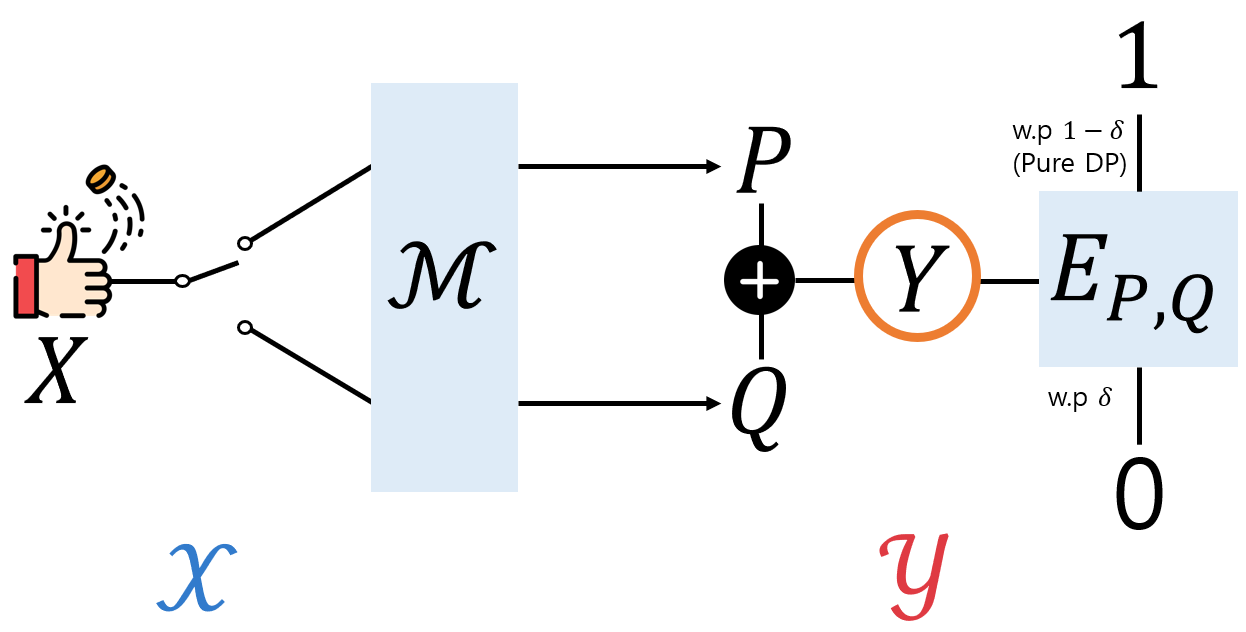
\includegraphics[width=1\linewidth]{Figure/5.6_visual.png}
    \caption{Visualization of the Bayesian version decomposition}
    \label{fig:decomposition}
\end{figure}
\section{Probability and Statistics}
\subsection{Moment}
\subsubsection{Moment and CDF}
For random variable $X$, 
\begin{equation}
    \E [X] = \int_0^{\infty} \pr (X \geq t) \dd{t} - \int_{-\infty}^0 \pr(X \leq t) \dd{t} 
\end{equation}
In general, $X \geq 0$ and a smooth function $g$ with $g(0) = 0 $  
\begin{equation}
    \E [g(X)] =\int_0^{\infty} g^{\prime} (t) P(X >t) \dd{t}  
\end{equation}
\subsubsection[alternative]{$k$-th moment in the lens of CDF}
\begin{equation}
    \frac{1}{k} \E[X^k] = - \int_{-\infty}^0 x^{k-1} F(x) \dd{x} + \int_0^{\infty} x^{k-1} (1- F(x)) \dd{x} 
\end{equation}
\subsubsection{Clipped random variable}
For complementary CDF $\bar{F}$ of random variable $X \geq 0$, 
\begin{equation}
    \E[\min(X,k)] = \int_0^k x f(x) \dd{x} + k \bar{F} (k), 
\end{equation}
\subsection{Conditional Distribution}
\alert{Tip:} ML/Statistics 분야에서 흔히 쓰는 notation $p(x|y), p(x,y)$ 같은 것은 $X,Y$ 들의 pdf/pmf라고 생각하자. 거의 measure는 안나옴. \\~\\
\header{Conditioning on event} 
Let $f_{X,Y}$ be the joint density of $X$ and $Y$, and $f_X (x)$ is the marginal density of $X$. 
\begin{enumerate}
    \item Single point conditioning $X=1$ 
    \begin{equation*}
        f_{Y | X=1} (y) = \frac{f_{X,Y} (1,y)}{f_{X} (1)} 
    \end{equation*}
    \item Set conditioning $X \in S$ 
    \begin{equation*}
    f_{Y | X \in S} (y) = \frac{\int_S f_{X,Y} (x,y) \dd{x}}{\int_S f_X (x) \dd{x}} = \frac{\int_S f_{Y | X=x}(y) f_X (x) \dd{x}}{\int_S f_{X} (x) \dd{x}}
    \end{equation*}
    \item Event conditioning 
    \begin{equation*}
        f_{Y |A} (y) = \frac{f_Y (y) \mathbf{1}[y \in A]}{\int_A f_Y (y) \dd{y}}
    \end{equation*}
 \end{enumerate}
\subsection{Weak convergence}
\subsubsection{Delta method}
If there is a sequence of random variables $X_n$ satisfying 
\begin{equation}
    \sqrt{n}[X_n - \theta] \weakly \cN(0, \sigma^2) 
\end{equation}
then 
\begin{equation}
    \sqrt{n}[g(X_n) - g(\theta)] \weakly \cN(0, \sigma^2 \cdot [g^{\prime}(\theta)]^2)
\end{equation}
given that $g^{\prime}(\theta)$ exists and is non-zero value. 
\subsubsection{Slutsky's theorem}
If $X_n$ converges in distribution to a random element $X$ and $Y_n$ converges in probability to a constant $c$, then 
\begin{enumerate}
    \item $X_n + Y_n \weakly X +c$ 
    \item $X_n Y_n \weakly Xc$ 
    \item$X_n / Y_n \weakly X/c$
\end{enumerate}
where $\weakly$ denotes convergence in distribution. 
\subsection{Central limit theorem}
\subsubsection{Salem-Zygmund}
\header{Theorem} Let $U$ be a uniform random variable with support $(0, 2\pi)$, and let $X_k = r_k \cos(n_k U + a_k) (0 \leq a_k < 2\pi)$, where 
\begin{enumerate}
    \item $n_k$ satisfy the \emph{lacunarity condition}: there exists $q>1$ such that $n_{k+1} \geq q n_k$ for all $k$ 
    \item $\sum_{i=1}^\infty r_i^2 = \infty$ and $\frac{r_k^2}{r_1^2 + \dots +r_k^2} \to 0$  
\end{enumerate}
Then, 
\begin{equation}
    \frac{X_1 + \dots +X_k}{\sqrt{r_1^2 + \dots + r_k^2}}
\end{equation}
converges in distribution to $\cN(0, 1/2)$. 
\subsection{Conditional independence}
\header{Theorem} Let $p_{X Y Z}$ be the joint PDF/PMF of $X,Y$ and $Z$. Then the following are equivalent with up to almost-everywhere equivalence:
\begin{enumerate}
    \item $X \perp Y \given Z$
    \item $p_{XY Z } (x,y,|z) = p_{X|Z}(x|z) p_{Y|Z}(y|z)$
    \item $p_{X|Y Z}(x|y,z) = p_{X|Z}(x|z)$
    \item $p_{XYZ}(x,y,z) = \frac{p_{XZ} (x,z) p_{YZ}(y,z)}{p_Z (z)}$
    \item $p_{XYZ} (x,y,z) = g(x,z) h(y,z)$ for some measurable functions $g$ and $h$
    \item $p_{X|Y Z} (x | y,z) = w(x,z)$ for some measurable function $w$ \\ 
\end{enumerate} 

\header{Properties} Let $X,Y,Z,W$ be RVs 
\begin{enumerate}
    \item (symmetry) $X \perp Y \given Z \iff Y \perp X \given Z$
    \item (decomposition) $X \perp Y \given Z \implies h(X) \perp Y \given Z$ for any measurable function $h$
    \item (weak union) $X \perp Y \given Z \implies X \perp Y \given Z, h(X)$ for any measurable function $h$ 
    \item (contraction) 
    \begin{equation}
        X \perp Y \given Z \mtext{and} X \perp W \given (Y,Z) \iff X \perp (W,Y) \given Z 
    \end{equation}
    \item If the joint PDF $P_{XYZW} (x,y,z,w)$ satisfies $f_{YZW} (y,z,w) >0$ almost everywhere. Then 
    \begin{equation}
        X \perp Y \given (W,Z) \mtext{and} X \perp W \given (Y,Z) \iff X \perp (W,Y) \given Z 
    \end{equation}
\end{enumerate}
\subsubsection{Bayes' Theorem}
Assume that $X$ is a random variable on $(\Omega, \cF, P)$,and let $Q$ be another probability measure on $(\Omega, \cF)$ with Radon-Nikodym derivative 
\begin{equation}
    L = \frac{\dd{Q}}{\dd{P}} \; \mtext{on} \cF
\end{equation}
Assume that $X \in L^1(\Omega, \cF, Q)$ and that $\cG$ is a sigma-algebra with $\cG \subseteq \cF$. Then 
\begin{equation}
    \E^Q [X \given \cG] = \frac{\E^P[L \cdot X \given \cG]}{\E^P [L \given \cG]}, \quad Q-a.s. 
\end{equation}
\subsubsection{Conditional expectation under independence}
\header{Proposition}
Let $(\Omega, \mathcal{B}, \prob)$ be a probability space, $(\mathbb{X}, \cM), (\mathbb{Y}, \cN)$ be measurable spaces, $X: \Omega \to X$ and $Y: \Omega \to \mathbb{Y}$ be measurable functions. If $X$ and $Y$ are \emph{independent} and $f \in (\cM \otimes \cN)_b$ then
\begin{equation}
    \E[f(X,Y) \given X] = \E[f(x,Y)] \rvert_{x=X} \; \text{a.s.}
\end{equation}
\subsection{Regular conditional distribution}  
\begin{figure}
    \centering
    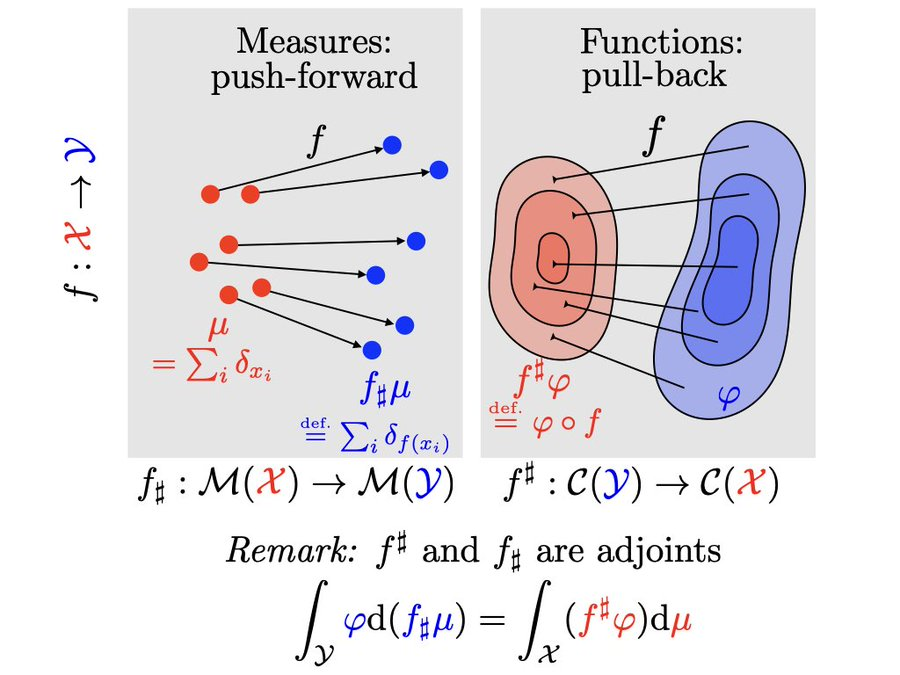
\includegraphics[width=0.75\linewidth]{Figure/dual_measure_function.png}
    \caption{Pullback of functions and pushforward of measures are dual one with each other!}
\end{figure}
\header{Theorem} If $X$ is a real random variable defined on probability space $(\Omega, \cF, \prob)$ then for every $\sigma$-algebra $\cG \subset \cF$ there is a regular conditional distribution for $X$ given $\cG$. \\~\\
Regular conditional distributions are useful in part because they allow one to reduce many
problems concerning conditional expectations to problems concerning only ordinary expectations. For such applications the following disintegration formula for conditional expectations
is essential. 
\subsubsection{Disintegration formula}
\header{Theorem} Let $\mu_w (\dd{x})$ be a regular conditional distribution for $X$ given $\cG$, let $Y$ be $\cG$-measurable, and let $f(x,y)$ be a jointly measurable real-valued function such that $\E[ |f (X,Y)|] < \infty$. Then, 
\begin{equation}
    \E[f(X,Y) \given \cG] = \int f(x, Y(w)) \mu_w (\dd{x}) \quad \mtext{a.s.}
\end{equation}
\header{Theorem2} Let $Y$ and $X$ be two Radon spaces. Let $\mu \in P(Y)$, let $\pi: Y \to X$ be a Borel-measurable function, and let $\nu \in P(X)$ be the pushforward measure from $Y$ to $X$ by $\pi$. Then there exists a $\nu$-almost everywhere uniquely determined family of probability measures $\set{\mu_x}_{x \in X} \subseteq P(Y)$ such that 
\begin{enumerate}
    \item the function $x \mapsto \mu_x$ is Borel measurable 
    \item $\mu_x$ lives on the fiber $\pi^{-1}(x)$
    \item for every Borel-measurable function $f: Y \to [0, + \infty]$, 
    \begin{equation}
        \int_Y f(y) \dd{\mu(y)} = \int_X \int_{\pi^{-1}(x)} f(y) \dd{ \mu_x(y)} \dd \nu(x) 
    \end{equation}
\end{enumerate}
\subsection{Markov kernel}
A Markov kernel (also called transition kernel, stochastic kernel, or probability kernel) is a mathematical formalization of a “function with random outcomes”.
\subsection{Mutual Information}
\subsubsection{Concavity of Mutual information}
Let $\alpha$ be the law of $X$ and $\pi$ be the conditions law of $Y|X$.  Let \( I_1 \) be \( I(X;Y) \) where \( (X,Y) \sim (\alpha_1, \pi) \),  
let \( I_2 \) be \( I(X;Y) \) where \( (X,Y) \sim (\alpha_2, \pi) \),  
let \( I \) be \( I(X;Y) \) where \( (X,Y) \sim (\lambda \alpha_1 + (1-\lambda) \alpha_2, \pi) \),  
for some \( 0 \leq \lambda \leq 1 \), then  
\[
I \geq \lambda I_1 + (1-\lambda) I_2.
\]
\subsection{Fisher Information}
Given the score function $\log p(\theta; X)$, the Fisher Information is defined as
\begin{equation}
    I(\theta) := \E_{\theta}\left[ - \frac{\partial^2}{\partial \theta^2} \log p(\theta; X)\right]
\end{equation}
It gives you uncertainty about the estimation since 
\begin{equation}
    \underbrace{\Var \left[ \frac{\partial \ell (\theta ; X)}{\partial \theta}\right]}_{\text{variance of score}} = - \E \left[ \frac{\partial^2 \ell(\theta ; X)}{\partial \theta^2} \right]
\end{equation}
holds. 
\subsubsection{Cramér–Rao bound}
Unbiased means there 
\begin{equation}
    \E[\hat{\theta}(X) - \theta \given \theta] = \int \left( \hat{\theta}(x) - \theta \right) f(x; \theta) \dd{x} = 0 \mtext{regardless of the value of} \theta
\end{equation}
Then, the following holds 
\begin{equation}
    \var(\hat{\theta}) \geq \frac{1}{I(\theta)}
\end{equation}
The precision to which we can estimate $\theta$ is fundamentally limited by the Fisher information of the likelihood function.
\subsection{MLE estimation}
\subsubsection{Asymptotic normality}
\begin{equation}
    \sqrt{n} (\hat{\theta}_n - \theta) \overset{D}{\rightarrow} \cN(0, I^{-1}(\theta))
\end{equation}
The mean square error (MSE) of $\hat{\theta}_n$ is 
\begin{equation}
    \text{MSE}(\hat{\theta}_n, \theta_0) = \text{bias}^2(\hat{\theta}) + \var (\hat{\theta}_n) \approx \frac{1}{n I(\theta_0)}
\end{equation}
Moreover, if we know about $I(\theta_0)$, we can construct a $1-\alpha$ confidence interval using 
\begin{equation}
    \left[ \hat{\theta}_n - \frac{z_{1-\alpha/2}}{\sqrt{n \hat{I}(\theta_0)}}, \hat{\theta}_n + \frac{z_{1- \alpha/2}}{\sqrt{n \hat{I}(\theta_0)}}\right] 
\end{equation}\footnote{CI: estimator $\pm$ z-value * (SD of estimator)}
\subsection{Famous Family}
\subsubsection{Poission}
\header{Binomial of Poisson trials is Poisson} Let $\lambda \geq 0, p \in [0,1]$. Suppose $(\red{X}_i)_{i=1}^{\infty}$ are i.i.d Bernoulli random variables with parameter $\red{p}$, and $N$ is a Poisson$(\lambda)$ random variable independent of the $\red{X}_i$'s. Then $\sum_{i=1}^N \red{X}_i \sim \text{Poi}(\lambda \red{p})$. \\~\\ 

\header{Tail Distribution} Let $X \sim \text{Poi}(\red{\lambda})$, for some parameter $\red{\lambda} > 0$. Then for any $\alert{x} >0$, we have 
\begin{equation}
    \pr [ X \geq \red{\lambda} + \alert{x}] \leq e^{- \frac{\alert{x}^2}{2\red{\lambda}} h \left( \frac{\alert{x}}{\red{\lambda}} \right)}
\end{equation}, 
and, for any $0 < \alert{x} < \red{\lambda}$, 
\begin{equation}
    \pr[ X \leq \red{\lambda} - \alert{x}] \leq e^{- \frac{\alert{x}^2}{2 \red{\lambda}} h \left( - \frac{\alert{x}}{\red{\lambda}} \right)}. 
\end{equation}
where $h(u) : = 2 \frac{(1+u) \log (1+u) -u }{u^2}$. In particular, this implies that for every $\alert{x} >0$, 
\begin{equation}
    \pr [ \abs{X - \red{\lambda}} \geq \alert{x}] \leq 2 e^{-\frac{\alert{x}^2}{2 (\red{\lambda} + \alert{x})}}. 
\end{equation}
\subsubsection{Binomial}
\header{Fact} If $X$ is Binomial$(n,p)$, then $\E[1 / (X+1)] \leq 1 / ((n+1)\cdot p ) $
\subsubsection{Negative Binomial}
\header{Negative binomial as a Poisson + logarithmic}
\begin{enumerate}
    \item Draw $\blue{T}$ from a Poisson distribution and draw $K_1, K_2, \dots, K_{\blue{T}}$ independently from a logarithmic distribution.
    \item Then $K = \sum_{t=1}^T K_t$ follows a negative binomial distribution. 
\end{enumerate}

\subsection{M-estimator}
\subsubsection{Consistency}
\header{Theorem} Suppose that 
\begin{enumerate}
    \item $\sup_{\theta \in \Theta} | M_n (\theta) - M(\theta)| \to 0$ in probability (ULLN)
    \item For all $\varepsilon >0$, $\sup \set{M(\theta): d(\theta, \theta_0) \geq \varepsilon} < M (\theta_0)$ (identifiability)  
    \item $M_n (\hat{\theta}_n) \geq M_n (\theta_0) - o_p (1)$
\end{enumerate}
Then $\hat{\theta}_n \to \theta_0$ in probability. 
\section{Convexity}
\subsection{Characterization}
Suppose $f: \real^n \to \real$ is twice differentiable over an open domain. Then, the following are equivalent
\begin{enumerate}
    \item $f$ is convex 
    \item $f(y) \geq f(x) + \nabla f(x)^{\top} (y-x)$, for all $x,y, \in \text{dom}(f)$
    \item $\nabla^2 f(x) \succeq 0$, for all $x \in \text{dom}(f)$
\end{enumerate}
여기서 Condition $3$은 모든 점에서 non-negative curvature를 가지고 있다는 의미. 
\subsubsection{Characterization of Strict Convexity}
\begin{enumerate}
    \item $\nabla^2 f(x) \succ  0$, $\forall \in \Omega$ ( The converse is not true) 
    \item A function $f$ is strictly convex on $\Omega \subseteq \real^n$ if and only if 
    \begin{equation*}
        f(y) > f(x) + \nabla^{\top} f(x) (y-x), \; \forall x,y, \in \Omega, x \neq y 
    \end{equation*}
    \item $f$ is strongly convex if and only if there exists $m>0$ such that 
    \begin{align*}
        &f(y) \geq f(x) + \nabla^{\top} f(x) (y-x) + m \norm{y-x}^2, \forall x,y, \in \text{dom}(f) \\ 
        &\iff  \nabla^2 f(x) \succeq m \mI, \forall x \in \text{dom}(f)
    \end{align*}
\end{enumerate}
\subsubsection{When can we assume equal variables?}
If the \alert{constraints and the function to be optimized are both symmetric with respect to a group of permutations of the variables}, then the solution set will also be symmetric with respect to this group.
\subsection{Dual Problem}
$g(\lambda, \nu) = \inf_{x \in \mathcal{D}} L(x, \lambda, \nu) $ is concave and lower bound of the optimal value.  \medskip

\header{Example} 
\begin{align*}
    \text{maxmize}\quad & \sum_{i=0}^m \prob_F [ F(t) = i ] \cdot \prob_{\check{W}} [\check{W}(t) \geq v -i ]  \\ 
    \text{subject to}\quad  & \sum_{i=0}^m \prob[F(t)=i] \cdot i \leq 2m \cdot \delta \\
    & \sum_{i=0}^m \prob_F [F(t) =i ] =1, \text{and} \prob_F [F(t) =i] \geq 0 \; \forall i \in \set{0, 1, \cdots, m} 
\end{align*}
\textbf{Step 1. Find Lagrangian}  
\begin{equation}
    L(F, \alpha, \beta, \lambda) = \sum_{i=0}^m \prob_F [ F(t) = i] (\prob_{\check{W}} [ \check{W}(t) \geq v- i] - \alpha i - \beta - \lambda_i)  + 2 m \delta \alpha + \beta 
\end{equation}
with $\alpha \geq  0, \lambda \geq 0.$ Then, $g(\alpha, \beta, \lambda) := \sup_F  L(F, \alpha, \beta, \lambda) \geq \sup_{F \in C} L(F, \alpha, \beta, \lambda) \geq f^*$.  To drop the first term, add the constraint: $\alpha \cdot i + \beta \geq \prob_{\check{W}} [\check{W} (t) \geq v-i]  \; \forall i \in \set{0,1, \cdots, m}$.  \\~\\
\textbf{Step 2. Optimize the Dual function}  
\begin{align*}
    \text{minimize} \quad & 2m \delta \alpha+ \beta  \\ 
    \text{subject to} \quad & \alpha \cdot i + \beta \geq \prob_{\check{W}} [\check{W} (t) \geq v -i] \quad \forall i \in \set{0,1, \dots, m} \\ 
    & \alpha \geq0 
\end{align*}
Make $\alpha,\beta$ as small as possible! 
\begin{align*}
    \beta &= \prob_{\check{W}^*} [ \check{W} \geq v], \\ 
    \alpha &= \max \left( \set{0} \cup \set{\frac{1}{i} \left( \prob_{\check{w}^*} [\check{W} \geq v-i] - \beta \right) : i \in \set{1,2, \cdots, m}} \right)
\end{align*}
where $\hat{W}^*$ is a distribution on $\real$ such that $\prob [ \check{W}^* \geq v-i] \geq \prob [\check{W} (t) \geq v-i]$ for all $i \in \set{0,1, \cdots, m}$ and all $t$ in the support of $T$.  \\~\\
\alert{Remark.} Dual problem을 구하는 과정에서 constraint 추가해도 괜찮음.

\section{Integral Technique}
\subsection{Gaussian Integral}
\subsubsection{Gauss-Hermite quadrature}
\begin{equation}
    \int_{-\infty}^{\infty} e^{-x^2/2} f(x)\dd{x} \approx  \sum_{i=1}^n w_i f(x_i)
\end{equation}
where $n$ is the number of sampled points used. The $x_i$ are the roots of the physicists' version of the Hermite polynomial $H_n (x) (i=1,2,\dots,n)$ and the associated weights $w_i$ are given by 
\begin{equation}
    w_i = \frac{2^{n-1}n! \sqrt{\pi}}{n^2[H_{n-1}(x_i)]^2}
\end{equation}

\subsubsection{Stein's lemma} 
For a differentiable function $\phi: \real \to \real$ with $\E_{x \sim \mathcal{N}(0, 1)} [ | \phi^{\prime} (x) | ] < \infty$
\begin{equation}
    \E_{x \sim \mathcal{N}(0,1)} [ \phi (x) x] = \E_{x \sim \mathcal{N}(0,1)} [ \phi^{\prime} (x)]
\end{equation}
\subsubsection{Change of measure}
\begin{equation}
    \cN(\vw | \vmu_n, \mSigma_n) \dd{\vw} = \cN(\vx^{\top} \vw | \vx^{\top} \mu_n, \vx^{\top} \mSigma_n \vx) \dd{(\vx^{\top} \vw)} 
\end{equation}
\section{Stochastic process}
\subsection{Predictable process}
\subsubsection{How to understand the predictable process?}
\header{Fact 1} The predictable sigma-algebra is generated by continuous and adapted processes. \\~\\
\header{Fact 2} The predictable sigma-algebra is generated by the sets of the form 
\begin{equation}
    \set{(s,t] \times A: t > x \geq 0 , A \in \cF_s} \cup \set{\set{0} \times A : A \in \cF_0}
\end{equation}
\subsection{Local martingale}
\subsubsection{Quadratic variation}
\header{Fact} If $X$ is a continuous local martingale, then $[X]_t < \infty$ a.s. for every $t \geq 0$, where $[X]$ denote the quadratic variation of the process $X$.  
\subsubsection{Stochastic integral}
\header{Proposition} For any continuous $L^2$-martingale $M$ where $M_0 =0 $, and any predictable step process $V$ where $|V| \leq 1$, the process $(V \cdot M)$ is an $L^2$-martingale with $\E (V \cdot M)_t^2 \leq \E M_t^2$. 
\subsection{Doob's h transform}
Set 
\begin{equation}
    h(x) = \prob_x (\tau_A < \tau_B)
\end{equation}
Then, $h(x)$ is the probability, starting from $x$ to hit $A$ before hitting $B$. Then $h$ is positive on $\mathcal{X} \setminus (A \cup B)$. Furthermore, for $x \notin A \cup B$ 
\begin{equation}
    \hat{P}(x,y) = \prob_x [X_1 = y | \tau_A < \tau_B]
\end{equation}
Finally, $h(x) =\prob_x ( \tau_A < \tau_B)$ satisfies both 
\begin{enumerate}
    \item $h(x) = 1 $ for $x \in A$ and $h(z) =0 $ for $z \in B$
    \item $h$ is harmonic at $x$ for every $x \notin A \cup B$ 
\end{enumerate}
and $h(\cdot)$ is the unique solution of linear system given by $1$ and $2$ above. \href{https://github.com/bellecp/CC-BY-SA-teaching-material/blob/master/stochastic_processes/homework-doob-h-transform-with-python-notebooks.pdf}{(Good source)}
\section{Fundamental Algebra}

\subsection{Series}
\subsubsection{Geometric}
\begin{equation}
    \sum_{n=a}^b r^n = r^a \frac{1-r^{b-a+1}}{1-r} = \frac{r^a - r^{b+1}}{1-r}
\end{equation}
\begin{equation}
    \sum_{j=1}^{\infty} \frac{j^2}{\rho^j} = \frac{\rho (\rho+1)}{(\rho-1)^3}
\end{equation}

\subsubsection{Quotient Stack}
\href{https://math.stackexchange.com/questions/384520/efficient-computation-of-sum-k-1n-left-lfloor-fracnk-right-rfloor}{(source)}
\begin{equation}
    \sum_{k=1}^n \floor{\frac{n}{k}} = 2 \sum_{k=1}^{\floor{\sqrt{n}}} \floor{\frac{n}{k}} - \floor{\sqrt{n}}^2    
\end{equation}

\subsection{Inequalities}
\subsubsection{Ratio of Summation}
\begin{equation}
    \frac{\sum_i a_i}{\sum_i b_i} \leq \max_i \frac{a_i}{b_i}
\end{equation}

\subsubsection{Weighted AM-GM Inequality}
Let the nonnegative numbers $x_1, x_2, \dots, x_n$ and the nonnegative weights $w_1, w_2, \dots w_n$ be given. Set $w = w_1 + w_2 + \dots w_n$. If $w>0$, then the inequality 
\begin{equation}
    \frac{w_1 x_1 +w_2 x_2 + \dots + w_n x_n}{w} \geq \sqrt[w]{x_1^{w_1}x_2^{w_2} \cdots x_n^{w_n}}
\end{equation}
holds.

\subsubsection{Titu's Lemma}
\header{Summation Form} For any real numbers $a_1, a_2, \dots a_n$ and positive reals $b_1, b_2, b_3, \dots b_n$, we have
\begin{equation}
    \frac{a_1^2}{b_1} + \frac{a_2^2}{b_2} + \dots + \frac{a_n^2}{b_n} \geq \frac{(a_1 + a_2 + \dots + a_n)^2}{b_1 + b_2 + \dots b_n}
\end{equation}

\header{Probabilistic Form} Let $X$ be a real random variable and $Y$ be a positive random variable such that $\E [|X|]$ and $\E[Y]$ are well defined. Then 
\begin{equation}
    \E[X^2/Y] \geq \E [|X|^2] / \E [Y] \geq \E[X]^2 / \E[Y]
\end{equation}

\subsubsection{Cauchy-Schwarz Inequality}
For any non-zero vector $\vx$, 
\begin{equation}
    \norm{\vx}_2^2 \leq \norm{\vx}_1^2 \leq \norm{\vx}_0 \norm{\vx}_2^2 
\end{equation}
(Note: Useful in binary matrix multiplication.)

\subsubsection{Chebyshev's Sum Inequality}
If $a_1 \geq a_2 \geq \cdots \geq a_n$ and $b_1 \geq b_2 \geq \cdots \geq b_n$, then
\begin{equation}
    \frac{1}{n} \sum_{k=1}^n a_k b_k \geq \left(\frac{1}{n} \sum_{k=1}^n a_k \right) \left( \frac{1}{n} \sum_{k=1}^n b_k \right) 
\end{equation}

\subsubsection{Symmetric Parametric Inequality}
\begin{equation}
 \left( 1- p + \frac{p}{x} \right)^{\alpha-2} \cdot (1- p + px)^{\alpha-2} \geq 1
\end{equation}
\subsubsection{We love Jensen}
By convexity of $(u,v) \mapsto u^{\lambda} v^{1-\lambda}$
\begin{equation}
    \E[U]^{\lambda} \E[V]^{1-\lambda } \leq \E[U^{\lambda} V^{1- \lambda}] 
\end{equation}
\subsection{Bounds and Approximations}
\subsubsection{Exponential Bound on Hyperbolic Ratio}
For $0 \leq y < x \leq 2$,
\begin{equation}
    \frac{\sinh(x) - \sinh(y)}{\sinh(x-y)} \leq e^{\frac{1}{2} x y}
\end{equation}

\subsubsection{Exponential Inequalities}
For all $t \in \real$ and $0 \leq p \leq 1$, 
\begin{equation}
    1-p + p \cdot x \leq e^{p (x-1)}
\end{equation}
Additionally:
\begin{equation}
    \forall x,y \geq 0  \quad \frac{1+e^{x+y}}{e^x + e^y} \leq e^{xy/2}
\end{equation}
\begin{equation}
    \frac{1}{2}(e^x + e^{-x}) \leq e^{x^2/2}
\end{equation}

\subsubsection{Softplus Quadratic Bound}
For all $a,x \in \real$ with $a \neq 0$, we have 
\begin{equation}
    \log(1+e^x) \leq \log(1+e^a) + \frac{x-a}{1+e^{-a}}+\frac{(e^a-1)\cdot(x-a)^2}{4\cdot a \cdot(e^a+1)}
\end{equation}

\subsubsection{Miscellaneous upper Bounds}
\header{Linear-Rational function}
For all $x > 0$, $t \in [0,1]$:
\begin{equation}
    \frac{1}{1-t +t x} \leq 1- t(1-t)(1+3t)(x-1) + t^2 \left( (1-t)x^2 + \frac{t}{x} -1 \right)
\end{equation} 
\header{Inverse logarithmic}
For all $u > 0$:
\begin{equation}
    \frac{1}{\log (1 + 1/u)} \leq u + \frac{1}{2}
\end{equation}
\header{$x \log_+ y$ decoupling}
For non negative reals $x$ and $y$, 
\begin{equation}
    x \log_+ y +1 \wedge +1 \leq x \log x + e^{-1} y + 1
\end{equation}
\header{Weighted reciprocal}
For all $p \in [0,1]$ and $x \in (0, \infty)$, 
\begin{equation}
    \frac{1}{1- p + p/x} \leq 1- p + p \cdot x 
\end{equation}
\subsubsection{Order of Rademacher Sums}
Let $\sigma \in \set{-1,1}^n$ be a random Rademacher sequence and let $a \in \real^n$ be an arbitrary real vector with sorted entries $\abs{a_1} \geq \abs{a_2} \geq \cdots \geq \abs{a_n}$. Then 
\begin{equation}
    \norm{\inner{a}{\sigma}}_{L^p} \sim \sum_{i \leq p} a_i + \sqrt{p} (\sum_{i > p} a_i^2 )^{1/2} 
\end{equation}

\subsubsection{Sum Approximation}
\begin{equation}
    \max(a,b) \leq a+b \leq 2 \max(a,b), \quad a,b \geq 0 
\end{equation}

\subsection{Combinatorics}
\subsubsection{Expansion}
\begin{equation}
    \binom{2n}{m} = \sum_{j=0}^{\floor{\frac{m}{2}}} \binom{n}{j} \binom{n-j}{m-2j} 2^{m-2j}
\end{equation}

\subsubsection{Vandermonde's Identity}
\begin{equation}
    \sum_{i=0}^r \binom{m}{i} \binom{n}{r-i} = \binom{n+m}{r}
\end{equation}
\begin{equation}
    \sum_{m=0}^n \binom{m}{j} \binom{n-m}{k-j} = \binom{n+1}{k+1} 
\end{equation}
Special form (\alert{hockey-stick identity}):
\begin{equation}
    \sum_{m=k}^n \binom{m}{k} = \binom{n+1}{k+1}
\end{equation}
(c.f. $\prod_{\ell=0}^{k-1} \left( \frac{\ell + \eta}{\ell +1} \right) = {k + \eta -1 \choose k})$

\section{Useful real analysis results}
\subsection{Leibniz's Integral Rule}  
Let $\mu$ be a probability distribution with support $\Omega$, let $I \subset \real$ be a nontrivial open interval, also let $f: \Omega \times I \to \real$ be a map with the following properties:
\begin{enumerate}
    \item For any $x \in I$, $\E_{w \sim \mu} [ | f(w,x) | ] < \infty$ (\alert{Uniformly finite moment}) 
    \item For almost all $w \in \infty$, the map $x \mapsto f(w,x)$ is differentiable with derivative $\frac{\partial}{\partial x} f(w, x)$ (\alert{differentiability}) 
    \item There is a map  $h: \Omega \to \real$ with the property that $\E_{w \sim \mu}  [ | h(w)|] < \infty$, such that $\abs{ \frac{\partial }{\partial x} f(\cdot, x) } \leq h$ (\alert{derivative bound}). 
\end{enumerate}
Then, for any $x \in I, E_{w \sim \mu} \left[ \abs{ \frac{\partial}{\partial x} f(w,x) } \right] < \infty$ and the function $F: x \to \E_{w \sim \mu} [f(w,x)] $ is differentiable with derivative 
\begin{equation}
    F'(x) = \E_{w \sim \mu} \left[ \frac{\partial}{\partial x} f(w,x) \right]
\end{equation}
\section{Linaer Algebra}

\subsection{Determinant}
\subsubsection{Expansion formula}
For any $A \subseteq \cY$, 
\begin{equation}
    \sum_{A \subseteq Y \subseteq \cY} \det(\mL_Y) = \det(\mL + \mI_{\bar{A}}), 
\end{equation}
\subsubsection{Rearrangement}
\begin{equation}
    \sum_{(I^{\prime}, J^{\prime}) \in \cS(I,J)} \det (\mZ_{Y, I^{\prime}}) \det (\mZ_{Y, J^{\prime}})  \leq \sum_{(I^{\prime}, *) \in \cS(I, j)} \det(\mZ_{Y, I^{\prime}})^2  
\end{equation}
where $\mI_{\bar{A}}$ is the diagonal matrix with ones in the diagonal positions with indices in $\bar{A}$ and zeros elsewhere. 
\subsubsection{Weinstein-Aronszajin identity}
If $\mA$ and $\mB$ are matrices of size $m \by n $ and $n \by m$ respectively, given that $\mA \mB$ is of trass class, then 
\begin{equation}
    \det(\mI + \mA \mB) = \det(\mI + \mB \mA)
\end{equation}
\subsubsection{DPP related}
\header{Propsosal matrix for NDPP} Given $\mV, \mB, \mD$ such that $\mL = \mV \mV^{\top} + \mB (\mD - \mD^{\top}) \mB^{\top}$, let $\set{\rho_i, \vv_i}_{i=1}^K$ be the eigendecomposition of $\mV \mV^{\top}$ and $\set{(\sigma_j, \vy_{2j-1}, \vy_{2j})}$ be the Youla decomposition of $\mB (\mD- \mD^{\top}) \mB^{\top}$. Denote $\mZ := [\vv_1, \dots, \vv_K, \vy_1, \dots, \vy_K] \in \real^{M \by 2K}$ and 
\begin{align*}
    \mX &:= \text{diag}\left(\rho, \dots, \rho_K, \begin{bmatrix}
        0 & \sigma_1 \\ 
        -\sigma_1 & 0 
    \end{bmatrix}, \dots 
    \begin{bmatrix}
        0 & \sigma_{K/2} \\ 
        -\sigma_{K/2} & 0 
    \end{bmatrix}
    \right), \\
    \hat{\mX} &:= \text{diag}\left(\rho, \dots, \rho_K, \begin{bmatrix}
        \sigma_1 & 0 \\ 
        0 & \sigma_1 
    \end{bmatrix}, \dots 
    \begin{bmatrix}
        \sigma_{K/2} & 0 \\ 
        0 & \sigma_{K/2} 
    \end{bmatrix}
    \right), 
\end{align*}
so that $\mL = \mZ \mX \mZ^{\top}$ and $\hat{\mL} = \mZ \hat{\mX} \mZ^{\top}$. Then, for every subset $\mY \subseteq [M]$, it holds that 
\begin{equation}
    \det (\mL_Y) \leq \det (\hat{\mL}_Y) 
\end{equation}
and the equality holds when the size of $\mY$ is equal to the rank of $\mL$. \\~\\
\header{Propsosal matrix for NDPP \RN{2}} 
Given $\mX \in \real^{n \by d}$ and $\mW^A \in \real^{d \by d}$ Then, 
\begin{equation}
    \det( [\mX \mW^A \mX^{\top}]_S ) \leq \det ( [ \mX \hat{\mW}^A \mX^{\top}]_S ) 
\end{equation}
for every $S \subseteq [n]$. In addition, equality holds when $|S| \geq d$.  \\~\\
\header{DPP probability expansion \citep[Lemma 2.6]{Kulesza2012DeterminantalPP}}
\begin{equation}
\pr_{\hat{\mL}}(Y) = \frac{\det (\hat{\mL}_Y)}{\det (\hat{\mL} + \mI)} = \sum_{E \subseteq[2K], |E| = |Y|} \det (\underbrace{\mZ_{Y,E} \mZ_{Y,E}^{\top}}_{\memo{elementary DPP}})  \prod_{i \in E} \frac{\lambda_i}{\lambda_i +1} \prod_{i \notin E} \frac{1}{\lambda_i +1} 
\end{equation}
\begin{enumerate}
    \item Choose an elementary DPP according to its mixture weight 
    \item Sample a subset from the selected elementary DPP \\
\end{enumerate}
\header{DPP probability expansion \RN{2}}
The probability of sampling $S \in \binom{n}{k}$ from the $k$-DPP with $\hat{\mL}$ can be decomposed into the following 
\begin{equation}
    \frac{\det (\hat{\mL}_S)}{e_k (\set{\lambda_i}_{i=1}^d)} = \sum_{E \in \binom{[d]}{k}} \frac{\prod_{i \in E} \lambda_i}{e_k ( \set{\lambda_i}_{i=1}^d)} \cdot \det (\mK_S^E) 
\end{equation}
where $\mK^E$ is a rank-$k$ projection matrix consisting of eigenvalues of $\hat{\mL}$. 
\subsubsection{Ratio}
Given that $\det (\mQ \mS \mQ^{\top}) \neq 0$
\begin{equation}
    \frac{\det (\mQ (\mS + \mR ) \mQ^{\top})}{\det (\mQ \mS \mQ^{\top})} \leq \det(\mI_2 + (\mQ \mS \mQ^{\top})^{-1/2} \mQ \mR \mQ^{\top} (\mQ \mS \mQ^{\top})^{-1/2})
\end{equation}
\subsubsection{Inverse of trace}
For an invertible matrix $\mA \in \real^{n \by n}$, 
\begin{equation}
    \tr({\mA^{-1}}) = \sum_{i=1}^n \det (\mA_{-i}) / \det (\mA),
\end{equation}
where $\mA_{-i} \in \real^{n-1 \by n-1}$ is the submatrix of $\mA$ where the $i$th row and column of $\mA$ are removed.  
\subsection{Vectorziation}
\begin{equation}
\vect(\mA \mX \mB) = (\mB^{\top} \otimes \mA) \vect(\mX) 
\end{equation}
\header{Lyapunov Equation}
\begin{align}
    \mA \mX + \mX \mB &= \mC \\ 
    \mA\mX\mI+\mI\mX\mB &= \mC \\ 
    (\mI \otimes \mA)\vect(\mX) + (\mB^{\top} \otimes \mI)\vect(\mX) &= \vect(\mC) \\ 
    \vect(\mX) &= (\mI \otimes \mA + \mB^{\top} \otimes \mI)^{-1} \vect(\mC) 
\end{align}
\subsection{Trace}
\begin{equation}
    \tr (\mA \mB \mC) = \vect(\mA^{\top})^{\top} (\mI \otimes \mB)\vect(\mC)
\end{equation}
\begin{equation}
    \tr (\mA^{\top} \mB \mC \mD^{\top}) = \vect(\mA)^{\top} (\mD \otimes \mB) \vect(\mC) 
\end{equation}
\subsubsection{Von Neumann's trace inequqality}
\header{Theorem} If $\mA, \mB$ are complex $n \by n$ matrices with singular values 
\begin{equation}
    \alpha_1 \geq \dots \geq \alpha_n , \quad \beta_1 \geq \dots \beta_n, 
\end{equation}
respectively, then 
\begin{equation}
    \abs{\tr(\mA\mB)} \leq \sum_{i=1}^n \alpha_i \beta_i 
\end{equation}
\subsection{Inversion}
\subsubsection{Woodbury identity}
\begin{equation}
    [\mA+\mB\mC\mD]^{-1} = \mA^{-1} - \mA^{-1} \mB [\mC^{-1}+\mD \mA^{-1} \mB]^{-1} \mD \mA^{-1}
\end{equation}
given that $\mA^{-1}$ and $\mC^{-1}$ exist.
If $\mB = \vx, \mC = \mI, \mD = \vy^{\top}$
\begin{equation}
    (\mA + \vx \vy^{\top})^{-1} = \mA^{-1} - \frac{(\mA^{-1} \vx)(\vy \mA^{-1})}{1+\vy^{\top} \mA^{-1} \vx}
\end{equation}
\subsubsection{Schur Complement}
Schur Complement essentially is a block Cholesky factorization of a matrix 
\begin{equation}
    \begin{bmatrix}
        \mA & \mB \\ 
        \mC & \mD  
    \end{bmatrix}
    = \begin{bmatrix}
        \mI & \mB \mD^{-1} \\ 
        \bm{0} & \mI 
    \end{bmatrix}
    \begin{bmatrix}
        (\mA - \mB \mD^{-1}\mC)  & \bm{0} \\ 
        \bm{0} & \mD 
    \end{bmatrix}
    \begin{bmatrix}
        \mI &  \bm{0} \\ 
        \mD^{-1} \mC & \mI 
    \end{bmatrix}
\end{equation}
$\mA - \mB \mD^{-1} \mA$ is called the \emph{Schur complement} of $\mD$.
\subsection{Hadamard Product}
\subsubsection{Quadratic Relation}
\begin{equation}
    \vx^{\top} (\mA \odot \mB) \vy = \tr(\text{Diag}(\vx) \mA \text{Diag}(\vy) \mB^{\top})
\end{equation}
By setting $\vx = \vy$, it shows that the Hadamard product of two PSD matrices is PSD. 
\subsubsection{Rank Relation}
\begin{equation}
    rank(\mA \odot \mB) \leq rank(\mA) rank (\mB) 
\end{equation}
\subsubsection{Spectrum Relation}
\begin{equation}
    \prod_{i=k}^n \lambda_i (\mA \odot \mB) \geq \prod_{i=k}^n \lambda_i (\mA \mB), \; \forall k=1, \dots, n 
\end{equation}
with $\lambda_i(\cdot)$ denotes PD matrix. 
\subsubsection{Determinant}
\begin{equation}
    \abs{\mA \odot \mB} \geq \abs{\mA} \abs{\mB}
\end{equation}
\subsection{Matrix Calculus}
\subsubsection{Matrix Chain rule}
\begin{equation}
    [\nabla_{\mX} f(g(\mX))]_{i j} = \sum_{k=1}^p \sum_{\ell=1}^q \frac{\partial f(G)}{\partial g_{k \ell}} \frac{\partial g_{k \ell}}{x_{i j }}
\end{equation}
\subsubsection{Differentials}
\begin{align}
    \dd{(\tr{\mX})} &= \tr{\dd{\mX}}
\\
    \dd{(\mX \otimes \mY}) &= (\dd{\mX}) \otimes \mY + \mX \otimes (\dd{\mY}) 
\\
    \dd{\mX^{-1}} &= - \mX^{-1} \cdot \dd{\mX} \cdot \mX^{-1}
\\
    \dd{(\det (\mX) )} &= \tr( \text{adj}(\mX) \dd{\mX}) 
\\
    \dd{\det (\mX)} &= \det(\mX) \tr(\mX^{-1} \dd{\mX}) 
\\
    \dd{\log(\det(\mX))} &= \tr(\mX^{-1} \dd{\mX}) 
\\ 
    \dd{\sigma(a)} &= (\text{Diag}(\sigma) - \text{Diag}(\sigma)^2) \dd{a}  
\\
    \dd{(\text{softmax}(\theta))} &= (\text{Diag}(\vy) - \vy \vy^{\top}) \dd{\theta}
\end{align}
Note: Elementwise function은 일단 Diagonal 형태로 바꿔서 생각해 보삼 ㅋ 
\subsubsection{Useful first derivatives}
\begin{align}
    \frac{\partial \tr{\mX}}{\partial \mX} &= \mI  
\\
    \frac{\partial \tr{\mX^{-1}}}{\partial \mX} &= -\mX^{-2} 
\\
\frac{\partial \tr(\mA \mX)}{\partial \mX} &= \mA^{\top}
\\
    \frac{\partial \tr( \mX^k)}{\partial \mX} &= {k \cdot (\mX^{\top})^{k-1}}
\\
    \frac{\partial \tr( \mX \mA \mX \mB)}{\partial \mX} &= \mB^{\top} \mX^{\top} \mA^{\top} + \mA^{\top} \mX^{\top} \mB^{\top}
\\
\frac{\partial \mA \mX^{-1} \mB}{\partial \mX} &= - \mX^{\top} \mA^{\top} \mB^{\top} \mX^{-\top} 
\\ 
\frac{\partial \log \det ( \mX)}{\partial \mX} &= \mX^{- \top}
\\
    \frac{\partial \det(\mX^{-1})}{\partial \mX} &= \frac{\mX^{- \top}}{\det{\mX}} 
\\ 
\frac{\partial \det(\mX^k)}{\partial \mX} &= k \det(\mX^k) \mX^{- \top} \\ 
\frac{\partial \log \det( \mX \mX^{\top})}{\partial \mX} &= 2 \mX [\mX^{\top} \mX]^{-1} \cdot \det(\mX \mX^{\top}) 
\\ 
\frac{\det( \mA \mX \mB)}{\partial \mX} &= \det(\mA \mX \mB) \mA^{\top} (\mA \mX \mB)^{-\top} \mB^{\top}
\end{align}
\subsubsection{Quadratic form}
\begin{align}
    \frac{\partial (\vx - \mA \vs)^{\top} \mW (\vx - \mA \vs)}{\partial \vs} &= - 2 \mA^{\top} \mW (\vx - \mA \vs) \\
    \frac{\partial (\vx - \vs)^{\top} \mW (\vx - \vs)}{\partial \vx} &= 2 \mW (\vx - \vs) \\ 
    \frac{\partial (\vx - \mA \vs)^{\top} \mW (\vs - \mA \vs)}{\partial \vx} &= 2 \mW (\vs - \mA \vs) \\
    \frac{\partial (\vx - \mA \vs)^{\top} \mW ( \vx - \mA \vs)}{\partial \mA} &= - 2 \mW (\vx - \mA \vs) \vs^{\top}
\end{align}
\subsubsection{Hessian product rule}
Given two functions $f,g: \real^n \to \real$, 
\begin{equation}
    H_c (fg) = (H_c f) g(c) + \nabla_c f^{\top} \nabla_c g + \nabla_c g^{\top} \nabla_c f + f(c) H_c g
\end{equation}
\subsubsection{Integration by parts}
Given vector valued function $\varphi$ and scalar function $f$ with vanishing condition, 
\begin{equation}
    \int_{\real^d} {\varphi (\vx) \cdot \nabla f (\vx) \dd{x}} = - \int_{\real^d} (\nabla \cdot \varphi(\vx)) f(\vx) \dd{x}  
\end{equation}
\subsection{Eigenvalues and Eigenvectors}
\subsubsection{General Properties}
Assume that $\mA \in \real^{n \by m}$ and $\mB \in \real^{m  \by n }$, 
\begin{align}
    \text{eig}(\mA\mB) &= \text{eig}(\mB\mA) \\ 
    \text{rank}(\mA) = r& \implies  \mtext{At most} r \mtext{non-zero} \lambda_i 
\end{align}
\subsubsection{Symmetric}
Assume $\mA$ is symmetric, then 
\begin{align}
    \mV \mV^{\top} &= \mI  \\ 
    \lambda_i &\in \real \\ 
    \tr(\mA^p) &= \sum_i \lambda_i^p \\
    \text{eig}(\mI + c \mA) &= 1 + c \lambda_i \\ 
    \text{eig}(\mA - c\mI) &= \lambda_i -c \\ 
    \text{eig}(\mA^{-1}) &= \lambda_i^{-1} 
\end{align}
For a symmetric, positive matrix $\mA$ 
\begin{equation}
    \text{eig}(\mA^{\top}\mA) = \text{eig}(\mA \mA^{\top}) = \text{eig}(\mA) \circ \text{eig}(\mA) 
\end{equation}
\subsubsection{Singular Value Decomposition}
Any $n \by m$ matrix $\mA$ can be written as 
\begin{equation}
    \mA = \mU \mD \mV^{\top}
\end{equation}
where 
\begin{align*}
    \mU &= \mtext{eigenvectors of} \mA\mA^{\top} \; n \by n \\
    \mD &= \sqrt{\text{diag} (\text{eig} (\mA \mA^{\top}))} \quad n \by m \\ 
    \mV &= \mtext{eigenvectors of} \mA^{\top}\mA \; m \by m 
\end{align*}
\header{Square decomposed into rectangular}
Assume $\mV_* \mD_* \mU_*^{\top} = 0 $ then we can expand the SVD of $\mA$ into 
\begin{equation}
    \mA = 
    \begin{bNiceArray}{c|c}[margin]
    \mV & \mV_* 
    \end{bNiceArray}
    \begin{bNiceArray}{c|c}[margin]
    \mD & \bm{0} \\ 
    \hline 
    \bm{0} & \mD_* 
    \end{bNiceArray}
    \begin{bNiceArray}{c}[margin]
        \mU^{\top} \\ 
        \hline 
        \mU_*^{\top}
    \end{bNiceArray}
\end{equation}
where the SVD of $\mA$ is $\mA = \mV \mD \mU^{\top}$
\subsubsection{LU decomposition}
Assume $\mA$ is a square matrix with non-zero leading prcinipal minors, then 
\begin{equation}
    \mA = \mL \mU 
\end{equation}
where $\mL$ is a unique unit lower triangular matrix and $\mU$ is a unique upper triangular matrix. 
\subsubsection{Cholesky decomposition}
Assume $\mA$ is a symmetric positive definite square matrix, then 
\begin{equation}
    \mA = \mU^{\top} \mU = \mL \mL^{\top}
\end{equation}
where $\mU$ is an unique upper triangular matrix and $\mL$ is a lower triangular matrix.
\subsubsection{Eigenvalues of its reverse}
\header{Proposition} Given $M \by K$ matrix $\mA, \mB$, the nonzero eigenvalues of $\mA \mB^{\top} \in \complex^{M \by M}$ and $\mB^{\top} \mA \in \complex^{K \by K}$ are identical. If addition, if $(\lambda, \vv)$ is an eigenpair of $\mB^{\top} \mA$ with $\lambda \neq 0$, then $(\lambda, \mA \vv / \norm{\mA \vv}_2)$ is an eigenpair of $\mA \mB^{\top}$.  
\subsubsection{Row stochastic matrix}
\label{sec:8.8.7}
\header{Fact} The operator norm of a row-stochastic matrix is $1$.  
\subsection{Inverses}
\subsubsection{Rank-1 update of the inverse of inner product}
Denote $\mA = (\mX^{\top} \mX)^{-1}$ and that $\mX$ is extended to include a new column vector in the end $\tilde{\mX} = [\mX, \vv]$, let $N = \vv^{\top} (\mI - \mX  \mA \mX^{\top})\vv$ then 
\begin{equation}
    (\tilde{\mX^{\top}}\tilde{\mX})^{-1} = 
    N^{-1}\begin{bmatrix}
    N \mA + \mA \mX^{\top} \vv (\mA \mX^{\top} \vv)^{\top} & - \mA \mX^{\top} \vv \\ 
    -\vv^{\top} \mX \mA^{\top} & 1 
    \end{bmatrix}
\end{equation}
\subsubsection{Approximations}
The following identity is known as the \emph{Neuman series} of a matrix, which holds when $\abs{\lambda_i} < 1$ for all eigenvalues $\lambda_i$
\begin{align}
    (\mI - \mA)^{-1} &= \sum_{n=0}^{\infty} \mA^n \\  
    (\mI + \mA)^{-1} &= \sum_{n=0}^{\infty} (-1)^n \mA^n 
\end{align}
\begin{align}
    \alert{\mA - \mA(\mI + \mA)^{-1} \mA}  &= \mA - \mA(\mI + \mA^{-1})^{-1} \\ 
    &= \mA(\mI - (\mI + \mA^{-1})^{-1})  \\ 
    &\approx \mA(\mI - \mI + \mA^{-1} - \mA^{-2}) \\ 
    &= \alert{\mI - \mA^{-1}}
\end{align}
\subsubsection{Block matrix}
Using Schur complements 
\begin{align}
    \mC_1 &= \mA_{11} - \mA_{12} \mA_{22}^{-1}\mA_{21} \\
    \mC_2 &= \mA_{22} - \mA_{21}\mA_{11}^{-1}\mA_{12} 
\end{align}
as 
\begin{align}
    \begin{bNiceArray}{c | c}[margin]
    \mA_{11} & \mA_{12} \\ 
    \hline 
    \mA_{21} & \mA_{22}  
    \end{bNiceArray}^{-1}
    &= 
    \begin{bNiceArray}{c | c}[margin]
    \mC_1^{-1} & -\mA_{11}^{-1} \mA_{12} \mC_2^{-1} \\ 
    \hline 
    -\mC_2^{-1} \mA_{21} \mA_{11}^{-1} & \mC_2^{-1}  
    \end{bNiceArray}
\end{align}
\subsection{PSD matrix}
\subsubsection{Decomposition}
\begin{enumerate}
    \item The matrix is PSD with rank $r$ $\iff$ there exists a matrix $\mB$ of rank $r$ such that $\mA = \mB \mB^{\top}$ 
    \item The matrix is PD $\iff$ there exists an invertible matrix $\mB$ such that $\mA = \mB \mB^{\top}$ 
    \item Given $\mA$ is an $n \by n $ PSD matrix, there exists an $n \by r$ matrix $\mB$ of rank $r$ such that 
    $\mB^{\top} \mA \mB = \mI$. 
\end{enumerate}
\subsubsection{Sylvester's characterization}
\begin{align}
    \mA \succeq 0 &\iff \mtext{All} 2^n -1 \mtext{principal minors are nonnegative.} \\ 
    \mA \succ 0 &\iff \mtext{All} n \mtext{leading principal minors are positive.}
\end{align}
\subsubsection{Eqution with zeros}
Assume $\mA$ is PSD, then $\mX^{\top} \mA \mX = \bm{0} \implies \mA \mX =0 $
\subsubsection{Rank of product}
Assume $\mA$ is positive definite, then $\text{rank}(\mB\mA\mB^{\top}) = \text{rank}(\mB)$  
\subsubsection{Outer product}
If $\mX \in n \by r$, where $n \leq r$ and $\text{rank}(\mX) = n$, then $\mX\mX^{\top}$ is positive definite. 
\subsubsection{Small pertubations}
If $\mA$ is positive definite, and $\mB$ is symmetric, then $\mA - t \mB$ is positive definite for sufficiently small $t$. 
\subsubsection{Hadamard inequality}
If $\mA$ is a positive definite or semi-definite matrix, then 
\begin{equation}
\det (\mA) \leq \prod_i A_{ii}
\end{equation}
\subsubsection{Loewner order}
\header{Fact} Let $\mA$ and $\mB$ be hermitian positive definite. Then 
\begin{equation}
    \mA \succeq \mB \iff \mI \succeq \mA^{-1/2} \mB \mA^{-1/2}
\end{equation}
\subsubsection{Inverse of PSD}
\header{Fact} Suppose that $\mA, \mB$ and $\mA - \mB$ are all positive definite, then $\mB^{-1} - \mA^{-1}$ is also positive definite.   
\subsection{Symmetric and skew-symmetric matrix}
\subsubsection{Properties of symmetric matrix}
\begin{enumerate}
    \item Every real symmetric matrix can be orthogonally diagonalizable. \footnote{Think of it this way: every symmetric matrix can be triangulated and normality is preserved under a similar transform. When is the triangular matrix normal? Of course, it is the diagonal matrix.} 
    \item  The rank of a symmetric matrix $\mA$ is equal to the number of non-zero eigenvalues of $\mA$.
    \item If $\mA$ and $\mB$ are $n \by n$ real symmetric matrices that commute, then they can be simultaneously diagonalized by an orthogonal matrix. 
\end{enumerate}
\subsubsection{Youla decomposition}
Given $\mB \in \real^{M \by K}$ and $D \in \real^{K \by K}$, consider a rank-$K$ skew-symmetric matrix $\mB^{\top} (\mD - \mD^{\top})\mB^{\top}$. Then, we can write 
\begin{align}
    \mB(\mD- \mD^{\top})\mB &= \sum_{j=1}^{K/2} i \sigma_j (\va_j + i \vb_j) (\va_j + i \vb_j)^H - i \sigma_j (\va-J - i \vb_j)(\va_j - i \vb_j)^H \\ 
    &= \sum_{j=1}^{K/2} 2 \sigma_j ( \va_j \vb_j^{\top} - \vb_j \va_j^{\top}) \\ 
    &= \sum_{j=1}^{K/2} 
    \begin{bmatrix}
        \va_j-\vb_j & \va_j + \vb_j 
    \end{bmatrix}
    \begin{bmatrix}
        0 & \sigma_j \\ 
        -\sigma_j & 0 
    \end{bmatrix}
    \begin{bmatrix}
        \va_j^{\top} - \vb_j^{\top} \\
        \va_j^{\top} + \vb_j^{\top} 
    \end{bmatrix}
\end{align}
Note that $\va_1 \pm \vb_1, \dots \va_{K/2} \pm \vb_{K/2}$ are real-valued orthonormal vectors. The pair $\set{(\sigma_j, \va_j - \vb_j , \va_j + \vb_j)}_{j=1}^{K/2}$ is often called the \alert{Youla decomposition} of $\mB (\mD - \mD^{\top})\mB^{\top}$.
\subsection{Some techniques}
\subsubsection{Binary analysis}
어떤 matrix의 operator norm을 분석하기 위해 matrix를 binary matrix로 decomposition하는 것은 유용할 수 있다.  \\~\\ 

\begin{ginzabox}[Example]
Let $\vv$ be the unit-normed vector that realizes the operator norm of $\mD^{-1} \mA$. We define the sequence of binary matrices $\mB^0, \mB^1, \mB^2$ as follows:
\begin{equation}
    B_{i,j}^t := \mathbf{1}_{\set{2^{-t-1}\sqrt{\alpha /n} < [\mD^{-1} \mA]_{i,j} \leq 2^{-t} \sqrt{\alpha/ n}}} \; \mtext{for every integers} t \geq 0,  
\end{equation}
where $\sqrt{\alpha/n}$ is the upper bound for entries of $\mD^{-1} \mA$.  Then we have the following inequalities for the entries and the $l_2$-norm: 
\begin{align}
    [\mD^{-1} \mA]_{i, j} &\leq \sqrt{\alpha /n } \sum_{t=0}^{\infty} 2^{-t} \cdot [\mB^t]_{i, j} \\ 
    \norm{\mD^{-1} \mA \cdot \vv}_2 &\leq \sqrt{\alpha /n} \sum_{t=0}^{\infty} 2^{-t} \cdot \norm{\mB^t \vv}_2 
\end{align}
만약 $\mB^t$ matrix의 row, column들의 non-zero elements를 estimate 하면 $\norm{\mB^t \vv}_2^2$도 estimate 할 수 있고 $\mD^{-1} \mA$의 operator norm의 bound도 estimate 할 수 있다.
\end{ginzabox}
\section*{Deferred proof}
\Cref{sec:8.8.7} 
Suppose $\mA \vx = \lambda \vx$ for some $\lambda >1$. Since the rows of $\mA$ are nonnegative and sum to $1$, each element of vector $\mA \vx$ is a convex combination of the components of $\vx$, which can be no greater than $\vx_{max}$. On the other hand, at least one element of $\lambda \vx$ is greater than $\vx_{max}$, which proves that $\vx_{max}$, which shows that $\lambda >1$ is impossible. 
\bibliography{references/citation}
\bibliographystyle{abbrv}
\end{document}
